\chapter{Appendix}
\section{Time calibration}
\label{chap:appendix time calibration}
\begin{figure}[H]
    \centering
    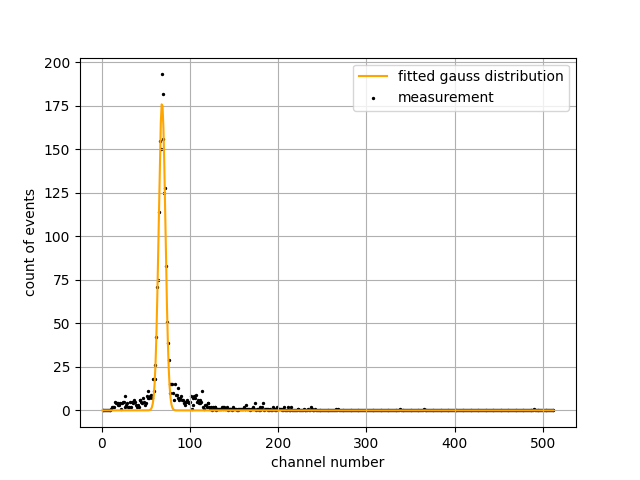
\includegraphics[width=110mm,scale=0.5]{Positronium/include/timecalibration0.png}
    \caption{Measured and fitted time spectrum at 0ns manual delay} 
    
\end{figure}

\begin{figure}[H]
    \centering
    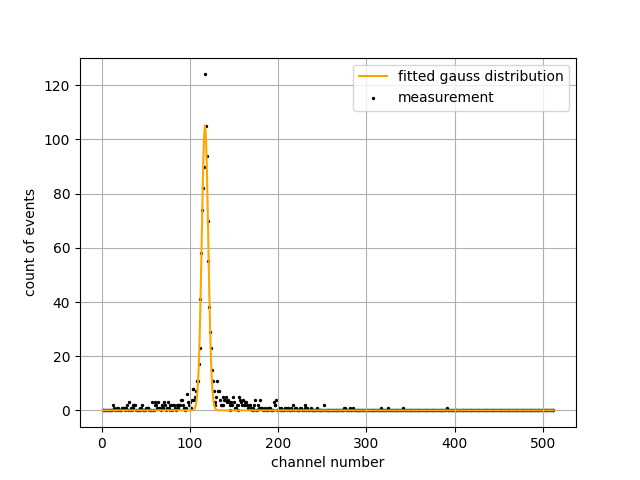
\includegraphics[width=110mm,scale=0.5]{Positronium/include/timecalibration1.png}
    \caption{Measured and fitted time spectrum at 4ns manual delay} 
   
\end{figure}

\begin{figure}[H]
    \centering
    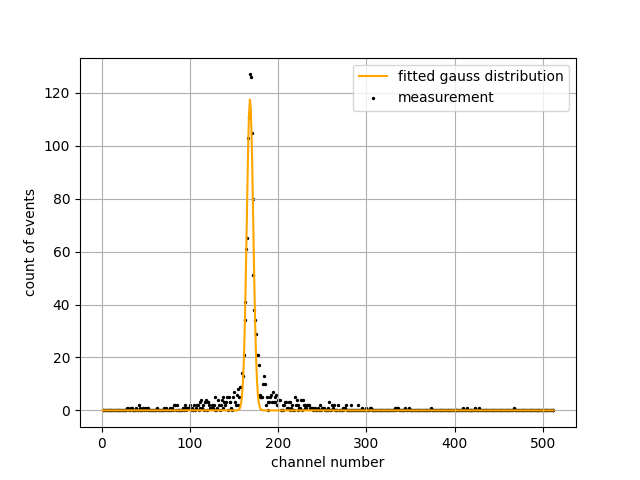
\includegraphics[width=110mm,scale=0.5]{Positronium/include/timecalibration2.png}
    \caption{Measured and fitted time spectrum at 8ns manual delay} 
   
\end{figure}

\begin{figure}[H]
    \centering
    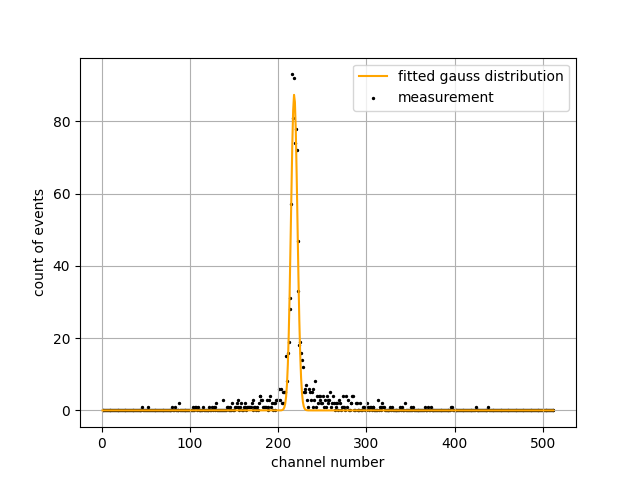
\includegraphics[width=110mm,scale=0.5]{Positronium/include/timecalibration3.png}
    \caption{Measured and fitted time spectrum at 12ns manual delay} 
    
\end{figure}

\begin{figure}[H]
    \centering
    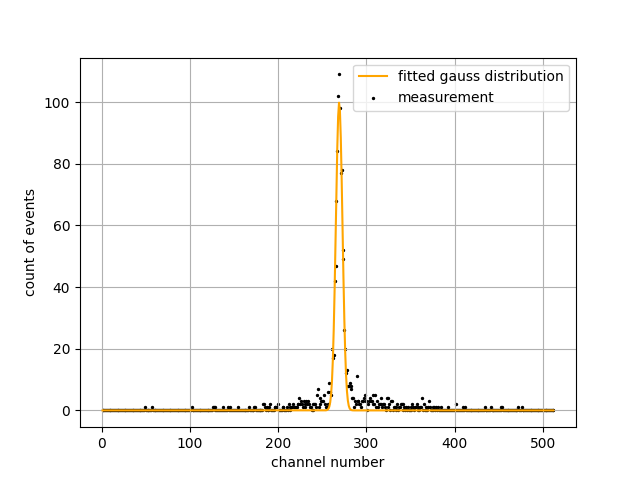
\includegraphics[width=110mm,scale=0.5]{Positronium/include/timecalibration4.png}
    \caption{Measured and fitted time spectrum at 16ns manual delay} 
   
\end{figure}

\begin{figure}[H]
    \centering
    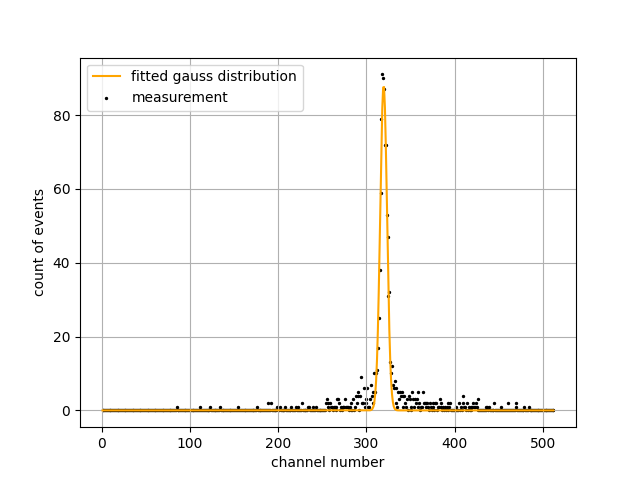
\includegraphics[width=110mm,scale=0.5]{Positronium/include/timecalibration5.png}
    \caption{Measured and fitted time spectrum at 20ns manual delay} 
   
\end{figure}

\begin{figure}[H]
    \centering
    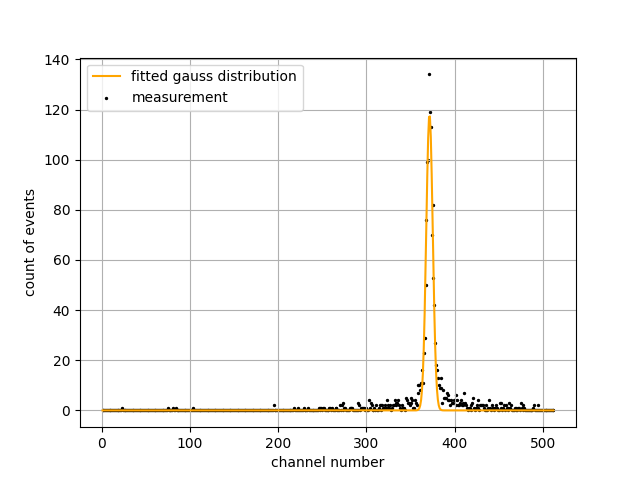
\includegraphics[width=110mm,scale=0.5]{Positronium/include/timecalibration6.png}
    \caption{Measured and fitted time spectrum at 24ns manual delay} 
   
\end{figure}

\begin{figure}[H]
    \centering
    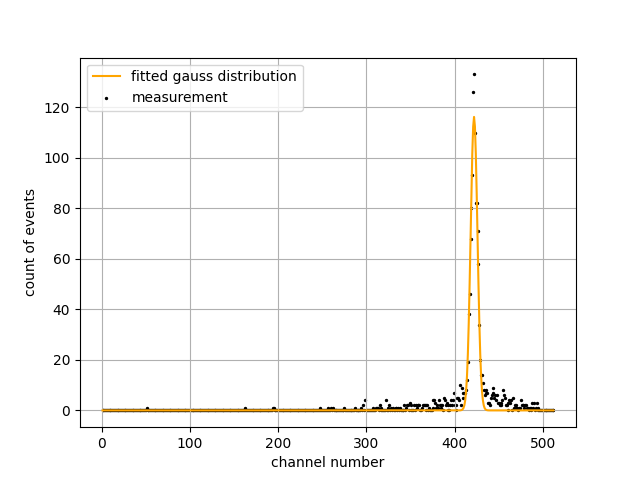
\includegraphics[width=110mm,scale=0.5]{Positronium/include/timecalibration7.png}
    \caption{Measured and fitted time spectrum at 28ns manual delay} 
   
\end{figure}

\begin{figure}[H]
    \centering
    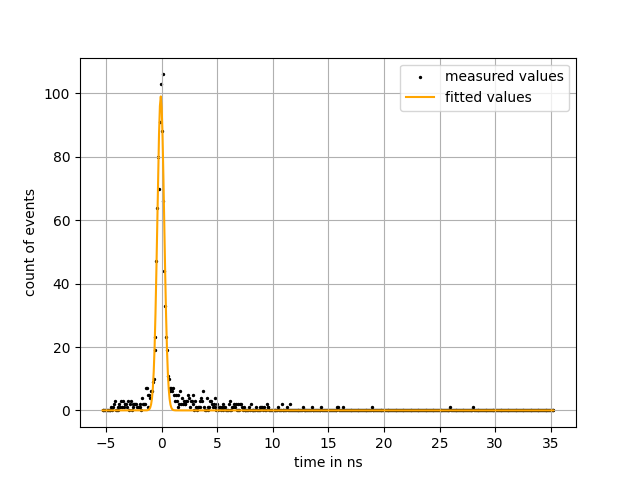
\includegraphics[width=110mm,scale=0.5]{Positronium/include/lightspeed fits0.png}
    \caption{Measured and fitted time spectrum at minimal distance} 
    
\end{figure}
\section{Speed of Light}
\label{chap:speedoflight}
\begin{figure}[H]
    \centering
    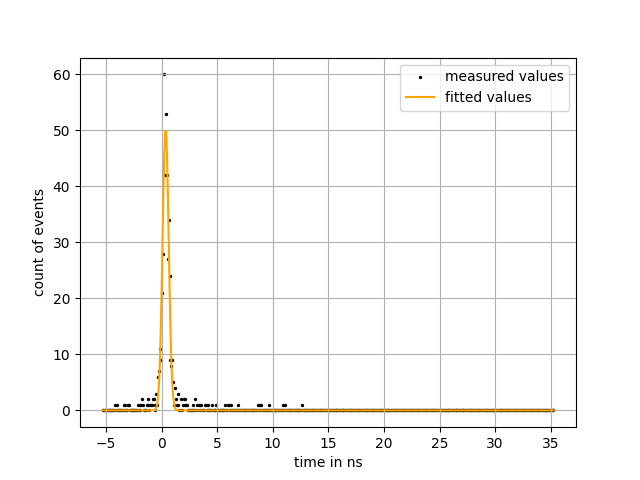
\includegraphics[width=110mm,scale=0.5]{Positronium/include/lightspeed fits1.png}
    \caption{Measured and fitted time spectrum at $d = \SI{10}{cm}$} 
    
\end{figure}
\begin{figure}[H]
    \centering
    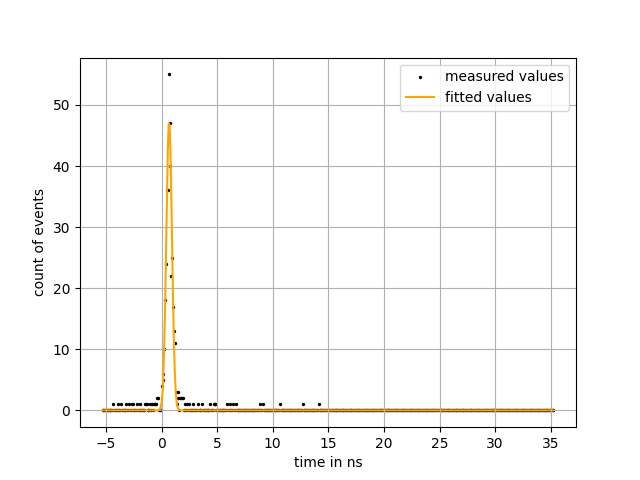
\includegraphics[width=110mm,scale=0.5]{Positronium/include/lightspeed fits2.png}
    \caption{Measured and fitted time spectrum  at $d = \SI{20}{cm}$} 
   
\end{figure}
\begin{figure}[H]
    \centering
    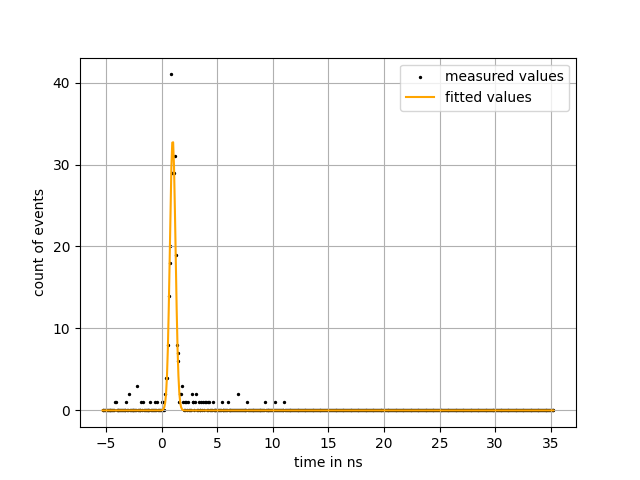
\includegraphics[width=110mm,scale=0.5]{Positronium/include/lightspeed fits3.png}
    \caption{Measured and fitted time spectrum  at $d = \SI{30}{cm}$} 
   
\end{figure}
\begin{figure}[H]
    \centering
    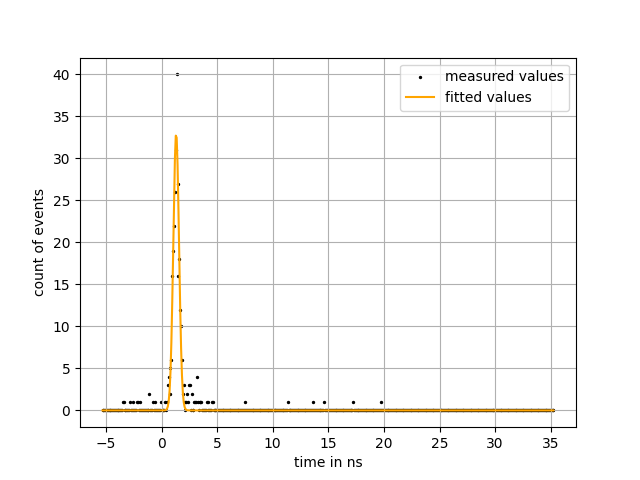
\includegraphics[width=110mm,scale=0.5]{Positronium/include/lightspeed fits4.png}
    \caption{Measured and fitted time spectrum  at $d = \SI{40}{cm}$} 
    
\end{figure}
\begin{figure}[H]
    \centering
    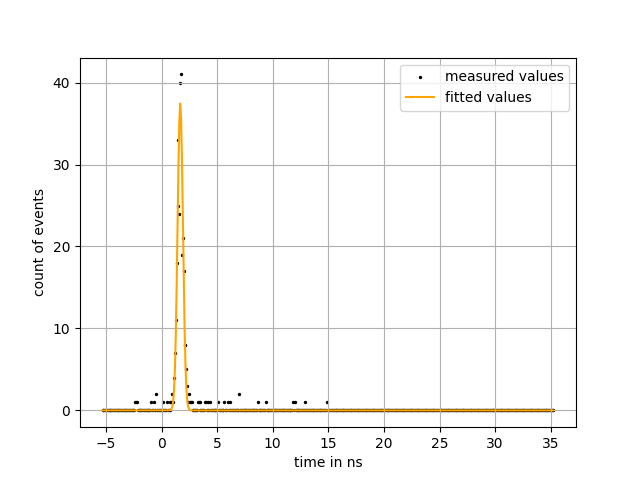
\includegraphics[width=110mm,scale=0.5]{Positronium/include/lightspeed fits5.png}
    \caption{Measured and fitted time spectrum at $d = \SI{50}{cm}$} 
   
\end{figure}

\begin{figure}[H]
    \centering
    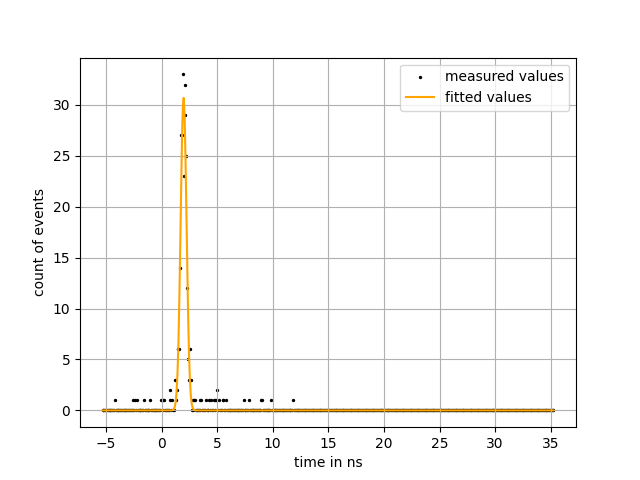
\includegraphics[width=110mm,scale=0.5]{Positronium/include/lightspeed fits6.png}
    \caption{Measured and fitted time spectrum at $d = \SI{60}{cm}$} 
   
\end{figure}